\documentclass[12pt, oneside]{article}

\usepackage[letterpaper, scale=0.89, centering]{geometry}
\usepackage{fancyhdr}
\setlength{\parindent}{0em}
\setlength{\parskip}{1em}

\pagestyle{fancy}
\fancyhf{}
\renewcommand{\headrulewidth}{0pt}
\rfoot{\href{https://creativecommons.org/licenses/by-nc-sa/2.0/}{CC BY-NC-SA 2.0} Version \today~(\thepage)}

\usepackage{amssymb,amsmath,pifont,amsfonts,comment,enumerate,enumitem}
\usepackage{currfile,xstring,hyperref,tabularx,graphicx,wasysym}
\usepackage[labelformat=empty]{caption}
\usepackage[dvipsnames,table]{xcolor}
\usepackage{multicol,multirow,array,listings,tabularx,lastpage,textcomp,booktabs}

\lstnewenvironment{algorithm}[1][] {   
    \lstset{ mathescape=true,
        frame=tB,
        numbers=left, 
        numberstyle=\tiny,
        basicstyle=\rmfamily\scriptsize, 
        keywordstyle=\color{black}\bfseries,
        keywords={,procedure, div, for, to, input, output, return, datatype, function, in, if, else, foreach, while, begin, end, }
        numbers=left,
        xleftmargin=.04\textwidth,
        #1
    }
}
{}
\lstnewenvironment{java}[1][]
{   
    \lstset{
        language=java,
        mathescape=true,
        frame=tB,
        numbers=left, 
        numberstyle=\tiny,
        basicstyle=\ttfamily\scriptsize, 
        keywordstyle=\color{black}\bfseries,
        keywords={, int, double, for, return, if, else, while, }
        numbers=left,
        xleftmargin=.04\textwidth,
        #1
    }
}
{}

\newcommand\abs[1]{\lvert~#1~\rvert}
\newcommand{\st}{\mid}

\newcommand{\A}[0]{\texttt{A}}
\newcommand{\C}[0]{\texttt{C}}
\newcommand{\G}[0]{\texttt{G}}
\newcommand{\U}[0]{\texttt{U}}

\newcommand{\cmark}{\ding{51}}
\newcommand{\xmark}{\ding{55}}

 
\begin{document}
\begin{flushright}
    \StrBefore{\currfilename}{.}
\end{flushright} 


\section*{Monday October 4}


Find and fix any and all mistakes with the following:
\begin{itemize}
\item[(a)] $(1)_2 = (1)_8$
\item[(b)] $(142)_{10} = (142)_{16}$
\item[(c)] $(20)_{10} = (10100)_2$
\item[(d)] $(35)_8 = (1D)_{16}$
\end{itemize} 

{\it Recall the definition of base expansion we discussed:}



{\bf Definition} For $b$ an integer greater than $1$ and $n$ a positive integer, 
the {\bf base $b$ expansion of $n$}  is
\[
(a_{k-1} \cdots a_1 a_0)_b
\]
where $k$ is a positive integer, $a_0, a_1, \ldots, a_{k-1}$ 
are nonnegative integers less than $b$, $a_{k-1} \neq  0$, and
\[
n =  \sum_{i=0}^{k-1} a_{i} b^{i}
\]

Notice: {\it The base $b$ expansion of a positive integer $n$ is a string over the alphabet 
$\{x \in \mathbb{N} \st x < b\}$
whose leftmost character is nonzero.}

\begin{center}
\begin{tabular}{|c|c|}
\hline
Base $b$ & Collection of possible coefficients in base $b$ expansion of  a positive integer \\
\hline
& \\
Binary ($b=2$) & $\{0,1\}$ \\
\hline
& \\
Ternary ($b=3$) & $\{0,1, 2\}$ \\
\hline
& \\
Octal ($b=8$) & $\{0,1, 2, 3, 4, 5, 6, 7\}$\\
\hline
& \\
Decimal ($b=10$) & $\{0,1, 2, 3, 4, 5, 6, 7, 8, 9\}$\\
\hline
& \\
Hexadecimal ($b=16$) &  $\{0,1, 2, 3, 4, 5, 6, 7, 8, 9, A, B, C, D, E, F\}$\\
& letter coefficient symbols represent numerical values $(A)_{16} = (10)_{10}$\\
&$(B)_{16} = (11)_{10} ~~(C)_{16} = (12)_{10} ~~
 (D)_{16} = (13)_{10} ~~ (E)_{16} = (14)_{10} ~~ (F)_{16} = (15)_{10} $\\
\hline
\end{tabular}
\end{center}

 
We write an algorithm for converting from base $b_1$ expansion to base $b_2$ expansion:

\phantom{
Earlier, we saw (two different) algorithms for, given 
a target base $b$, converting from decimal to base $b$ expansions. 
We will use either one of these as a subroutine in this algorithm.\\
Given a base expansion in base $b_1$:\\
Step 1: Use the definition of base expansion to calculate the value of
    this number (in decimal).\\
Step 2: Use the Least Significant First algorithm to write this value in 
    base $b_2$ and output the result.
}
\vspace{200pt} 

{\bf Definition} For $b$ an integer greater than $1$, $w$ a positive integer, 
and $n$ a nonnegative integer
$\underline{\phantom{\hspace{1in}}}$, ~
the {\bf base $b$ fixed-width $w$ expansion of $n$}  is
\[
(a_{w-1} \cdots a_1 a_0)_{b,w}
\]
where  $a_0, a_1, \ldots, a_{w-1}$ are nonnegative integers less than $b$ and
\[
n =  \sum_{i=0}^{w-1} a_{i} b^{i}
\]
 

\begin{center}
    \begin{tabular}{|c|c|c|c|c|}
    \hline
    Decimal &  Binary  & Binary fixed-width $10$& Binary fixed-width $7$ & Binary fixed-width $4$\\
    $b=10$ & $b=2$ & $b=2$, $w =  10$& $b=2$, $w =  7$& $b=2$, $w =  4$ \\
    \hline 
    &&&&  \\
    $(20)_{10}$&\phantom{$(10100)_{2}$\qquad\qquad}&&  &\\
    &&&&  \\
    &(a)&(b)&(c)&(d)  \\
    \hline
    \end{tabular}
    \end{center}
 

{\bf Definition} For $b$ an integer greater than $1$, $w$ a positive integer, 
$w'$ a positive  integer, and $x$ a real number the {\bf base $b$ fixed-width 
expansion of $x$ with integer part width $w$  and fractional part width $w'$} is
$(a_{w-1} \cdots a_1 a_0 .  c_{1} \cdots c_{w'})_{b,w,w'}$
where  $a_0, a_1, \ldots, a_{w-1}, c_1, \ldots, c_{w'}$ are nonnegative integers less than $b$ and
$$x \geq \sum_{i=0}^{w-1} a_{i} b^{i} + \sum_{j=0}^{w'}  c_{j} b^{-j} \hfill
\textrm{\qquad and \qquad}
\hfill x < \sum_{i=0}^{w-1} a_{i} b^{i} + \sum_{j=1}^{w'} c_{j} b^{-j} + b^{-w'}$$

\begin{center}
\begin{tabular}{|c|p{5in}|}
\hline
& \\
$3.75$  in fixed-width binary,& \\
integer part width $2$,&\\
 fractional part width $8$ & \\
& \\
\hline
& \\
$0.1$  in fixed-width binary, & \\
integer part width $2$, &\\
 fractional part width $8$ & \\
& \\
\hline
\end{tabular}
\end{center}

\includegraphics[width=2in]{../../resources/images/ArithmeticDemo.png}

Note: Java uses floating point, not fixed width representation, but similar rounding errors appear in both.
 
\newpage
\subsection*{Review: Week 2 Monday}
\begin{enumerate}
    \item {

Recall the definitions from class for number representations for {\bf base $b$ expansion of $n$},
{\bf  base $b$ fixed-width $w$ expansion of $n$}, and {\bf base $b$ fixed-width expansion of $x$ 
with integer part width $w$ and fractional part width $w'$}.

For example, the base $2$ (binary) expansion of $4$ is 
$\qquad
(100)_2 \qquad$
and the base $2$ (binary) fixed-width $8$ expansion of $4$ is
$\qquad
(00000100)_{2,8} \qquad$
and the base $2$ (binary) fixed-width expansion of $4$ with integer part width $3$ and fractional
part width $2$ of $4$ is
$\qquad
(100.00)_{2,3,2} \qquad$

Compute the listed expansions.  Enter your number using the notation for base 
expansions with parentheses but without subscripts. For example, 
if your answer were $(100)_{2,3}$
you would type \texttt{(100)2,3} into Gradescope.

\begin{enumerate}
\item Give the binary (base $2$) expansion of the number whose octal (base $8$) expansion is
\[
(371)_8
\]
\item Give the decimal (base $10$) expansion of the number whose octal (base $8$) expansion is
\[
(371)_8
\]
\item Give the octal (base $8$) fixed-width $3$ expansion of $(9)_{10}$?
\item Give the ternary (base $3$) fixed-width $8$ expansion of $(9)_{10}$?
\item Give the hexadecimal (base $16$) fixed-width $6$ expansion of
$(16711935)_{10}$?\footnote{This matches a frequent debugging task --
sometimes a program will show a number formatted as a base $10$
integer that is much better understood with another representation.}
\item Give the hexadecimal (base $16$) fixed-width $4$ expansion of
$$(1011~ 1010 ~ 1001~ 0000 )_2$$
Note: the spaces between each group of 4 bits above are for your convenience only.  How
might they help your calculations?
\item Give the binary fixed width expansion of $0.125$ with integer part width $2$ and 
fractional part width $4$.
\item Give the binary fixed width expansion of $1$ with integer part width $2$ and 
fractional part width $3$.
\end{enumerate} }
    \item {

Select all and only the correct choices below.
\begin{enumerate}
\item Suppose you were told that the positive integer $n_1$ has the property that $n_1 \textbf{ div } 2 = 0$. Which of the following can you conclude?
\begin{enumerate}
\item $n_1$ has a binary (base $2$) expansion
\item $n_1$ has a ternary (base $3$) expansion
\item $n_1$ has a hexadecimal (base $16$) expansion
\item $n_1$ has a base $2$ fixed-width $1$ expansion
\item $n_1$ has a base $2$ fixed-width $20$ expansion
\end{enumerate}
\item Suppose you were told that the positive integer $n_2$ has the property that $n_2 \textbf{ mod } 4 = 0$. Which of the following can you conclude?
\begin{enumerate}
\item the leftmost symbol in the binary (base $2$) expansion of $n_2$ is $1$
\item the leftmost symbol in the base $4$ expansion of $n_2$ is $1$
\item the rightmost symbol in the base $4$ expansion of $n_2$ is $0$
\item the rightmost symbol in the octal (base $8$) expansion of $n_2$ is $0$
\end{enumerate}
\end{enumerate} }
\end{enumerate}
\newpage
\section*{Wednesday October 6}


\begin{center}
    \begin{tabular}{|p{3.7in}|p{3.7in}|}
    \hline 
    &   \\
    {\bf base $b$ expansion of $n$}  & {\bf base $b$ fixed-width $w$ expansion of $n$}  \\
    & \\
    \hline  
    For $b$ an integer greater than $1$ and $n$ a positive integer, 
    the {\bf base $b$ expansion of $n$}  is $(a_{k-1} \cdots a_1 a_0)_b$
    where $k$ is a positive integer, $a_0, a_1, \ldots, a_{k-1}$ are nonnegative integers 
    less than $b$, $a_{k-1} \neq  0$, and $n =  a_{k-1} b^{k-1} + \cdots + a_1b + a_0$
    & 
    For $b$ an integer greater than $1$, $w$ a positive integer, and $n$ a nonnegative integer
    with $n <  b^w$, the {\bf base $b$ fixed-width $w$ expansion of $n$}  is
    $(a_{w-1} \cdots a_1 a_0)_{b,w}$
    where  $a_0, a_1, \ldots, a_{w-1}$ are nonnegative integers less than $b$ and 
    $n =  a_{w-1} b^{w-1} + \cdots + a_1b + a_0$\\
    \hline
    \end{tabular}
\end{center} 

{\bf Representing negative integers in binary}: Fix a positive integer  width for the representation  $w$, $w >1$.

\begin{tabular}{|cc|p{3.4in}|p{3.7in}|}
\hline
& & To  represent a positive integer $n$ & To represent a negative integer $-n$\\
\hline
&& &  \\
&\parbox[t]{2mm}{\multirow{4}{*}{\rotatebox[origin=c]{90}{Sign-magnitude}}} &
$[ 0a_{w-2} \cdots a_0]_{s,w}$, where $n =  (a_{w-2} \cdots a_0)_{2,w-1}$& 
$[1a_{w-2} \cdots a_0]_{s,w}$
, where $n =  (a_{w-2} \cdots a_0)_{2,w-1}$\\
&& & \\
&& Example $n=17$, $w=7$:  & Example $-n=-17$, $w=7$: \\
&& & \\
&& & \\
&& & \\
&& & \\
&& & \\
&& & \\
&& & \\
\hline
&&  &  \\
&\parbox[t]{2mm}{\multirow{4}{*}{\rotatebox[origin=c]{90}{2s complement}}} &
$[0a_{w-2} \cdots a_0]_{2c,w}$, where $n =  (a_{w-2} \cdots a_0)_{2,w-1}$& $[1a_{w-2} \cdots a_0]_{2c,w}$, where $2^{w-1} - n =  (a_{w-2} \cdots a_0)_{2,w-1}$\\
&& & \\
&& Example $n=17$, $w=7$:  & Example $-n=-17$, $w=7$: \\
&& & \\
&& & \\
&& & \\
&& & \\
&& & \\
&& & \\
&& & \\
\hline
&&  &  \\
\parbox[t]{1.5mm}{\multirow{4}{*}{\rotatebox[origin=c]{90}{{\it Extra example:}}}} 
& \parbox[t]{2mm}{\multirow{4}{*}{\rotatebox[origin=c]{90}{1s complement}}} &
$[0a_{w-2} \cdots a_0]_{1c,w}$, where $n =  (a_{w-2} \cdots a_0)_{2,w-1}$& $[1\bar{a}_{w-2} \cdots \bar{a}_0]_{1c,w}$, where $n =  (a_{w-2} \cdots a_0)_{2,w-1}$ and we define  $\bar{0} = 1$ and $\bar{1} = 0$.\\
&& & \\
&& Example $n=17$, $w=7$:  & Example $-n=-17$, $w=7$: \\
&& & \\
&& & \\
&& & \\
&& & \\
&& & \\
\hline
\end{tabular} \newpage


For positive integer $n$, to represent $-n$ in 
$2$s complement with width $w$,
\begin{itemize}
    \item Calculate $2^{w-1} - n$, convert 
    result to binary fixed-width $w-1$, pad 
    with leading $1$, or
    \item Express $-n$ as a sum of powers of $2$, 
    where the leftmost $2^{w-1}$ is negative weight, or
    \item Convert $n$ to binary fixed-width, 
    flip bits, add 1 (ignore overflow)
\end{itemize}

{\it Challenge: use definitions to explain why
each of these approaches works.} 

{\bf Representing $0$}:

So far, the definitions of base expansions treat
positive and negative integers. What about $0$?

\begin{tabular}{|cc|p{3.4in}|p{3.7in}|}
   \hline
   & & To  represent a {\bf non-negative} integer $n$ & To represent a {\bf non-positive} integer $-n$\\
   \hline
   && &  \\
   &\parbox[t]{2mm}{\multirow{4}{*}{\rotatebox[origin=c]{90}{Sign-magnitude}}} &
   $[ 0a_{w-2} \cdots a_0]_{s,w}$, where $n =  (a_{w-2} \cdots a_0)_{2,w-1}$& 
   $[1a_{w-2} \cdots a_0]_{s,w}$
   , where $n =  (a_{w-2} \cdots a_0)_{2,w-1}$\\
   && & \\
   && Example $n=0$, $w=7$:  & Example $-n=0$, $w=7$: \\
   && & \\
   && & \\
   && & \\
   && & \\
   && & \\
   && (a) & (b)\\
   \hline
   &&  &  \\
   &\parbox[t]{2mm}{\multirow{4}{*}{\rotatebox[origin=c]{90}{2s complement}}} &
   $[0a_{w-2} \cdots a_0]_{2c,w}$, where $n =  (a_{w-2} \cdots a_0)_{2,w-1}$& $[1a_{w-2} \cdots a_0]_{2c,w}$, where $2^{w-1} - n =  (a_{w-2} \cdots a_0)_{2,w-1}$\\
   && & \\
   && Example $n=0$, $w=7$:  & Example $-n=0$, $w=7$: \\
   && & \\
   && & \\
   && & \\
   && & \\
   && & \\
   && (c) & (d) \\
   \hline
\end{tabular} \newpage


{\bf Fixed-width addition}: adding one bit at time, using the usual column-by-column and carry arithmetic, and dropping the carry from the leftmost column so the result is the same width as the summands.  {\it Does this give the right value for the sum?}
\begin{multicols}{3}
\begin{align*}
   & (1~ 1~ 0~ 1~ 0~ 0)_{2,6}\\
+ & (0~ 0~ 0~ 1~ 0~ 1)_{2,6}\\
&\overline{\phantom{(1~1~1~0~0~1)_{2,6}}}\\
\end{align*}

\begin{align*}
   & [1~ 1~ 0~ 1~ 0~ 0]_{s,6}\\
+ & [0~ 0~ 0~ 1~ 0~ 1]_{s,6}\\
&\overline{\phantom{(1~1~1~0~0~1)_2}}\\
\end{align*}

\begin{align*}
   & [1~ 1~ 0~ 1~ 0~ 0]_{2c,6}\\
+ & [0~ 0~ 0~ 1~ 0~ 1]_{2c,6}\\
&\overline{\phantom{(1~1~1~0~0~1)_2}}\\
\end{align*}
\end{multicols} \newpage
\subsection*{Review: Week 2 Wednesday}
\begin{enumerate}
    \item {

Recall the definitions of signed integer representations from class: 
sign-magnitude and 2s complement.

\begin{enumerate}
    \item Give the 2s complement width 6 representation of the number 
    represented in binary fixed-width 5
    representation as $(00101)_{2,5}$. 
    \item Give the 2s complement width 6 representation of the number 
    represented in binary fixed-width 5
    representation as $(10101)_{2,5}$. 
    \item Give the 2s complement width 4 representation of the number 
    represented in sign-magnitude
    width 4 as $[1111]_{s,4}$.
    \item Give the sign magnitude width 4 representation of the number 
    represented in 2s complement
    width 4 as $[1111]_{2c,4}$.
    \item Give the sign magnitude width 6 representation of the number 
    represented in sign magnitude width 4 as $[1111]_{s,4}$.
    \item Give the 2s complement width 6 representation of the number 
    represented in 2s complement width 4 as $[1111]_{2c,4}$.
\end{enumerate} }
    \item {

Recall the definitions of signed integer representations from class: 
sign-magnitude and 2s complement.

\begin{enumerate}
    \item In binary fixed-width addition (adding one bit at time, using 
    the usual column-by-column and carry arithmetic, and ignoring the carry 
    from the  leftmost column), we get: 
    \begin{align*}
        &1110  \qquad  \text{first summand}\\
        +&0100 \qquad  \text{second summand}\\
        &\overline{0010} \qquad \text{result}
    \end{align*}
    Select all and only the  true  statements below:
    \begin{enumerate}
        \item When interpreting each of the summands and the result in binary fixed-width 4, 
        the result represents the actual value of the sum of the summands.
        \item When interpreting each of the summands and the sum in sign-magnitude width 4, the result  
        represents the actual value of the sum of the summands.
        \item When interpreting each of the summands and the sum in 2s complement width 4, the result 
        represents the actual value of the sum of the summands.
    \end{enumerate}    
    \item In binary fixed-width addition (adding one bit at time, using the 
    usual column-by-column and carry arithmetic, and ignoring the carry from the 
    leftmost column), we get: 
    \begin{align*}
        &0110  \qquad  \text{first summand}\\
        +&0111 \qquad  \text{second summand}\\
        &\overline{1101} \qquad \text{result}
    \end{align*}
    Select all and only the  true  statements below:
    \begin{enumerate}
        \item When interpreting each of the summands and the result in binary fixed-width 4, 
        the result represents the actual value of the sum of the summands.
        \item When interpreting each of the summands and the sum in sign-magnitude width 4, 
        the result  
        represents the actual value of the sum of the summands.
        \item When interpreting each of the summands and the sum in 2s complement width 4, 
        the result 
        represents the actual value of the sum of the summands.
    \end{enumerate}   
\end{enumerate} }
\end{enumerate}
\newpage
\section*{Friday October 8}


In a {\bf combinatorial circuit} (also known as
a {\bf logic circuit}), we have {\bf logic gates} 
connected
by {\bf wires}. The inputs to the circuits are the 
values set on the input wires: possible
values are 0 (low) or 1 (high). The values
flow along the wires from left to right.
A wire may be split into two or more wires, 
indicated with a filled-in circle (representing
solder). Values stay the same along a wire. When 
one or more wires flow into a gate, the output 
value of that gate is computed
from the input values based on the gate's definition
table. Outputs of gates may become inputs to other
gates.  

\begin{multicols}{2}
\begin{center}\begin{tabular}{cc|c}
Inputs &  & Output \\
$x$ & $y$ & $x \text{ AND } y$  \\
\hline
$1$ & $1$ & $1$\\
$1$ & $0$ & $0$\\
$0$ & $1$ & $0$\\
$0$ & $0$ & $0$\\
\end{tabular}\end{center}
\columnbreak
\begin{center}\includegraphics[height=0.6in]{../../resources/images/xANDy.png} \end{center}
\end{multicols}

\begin{multicols}{2}
\begin{center}\begin{tabular}{cc|c}
Inputs &  & Output \\
$x$ & $y$ & $x \text{ XOR } y$  \\
\hline
$1$ & $1$ & $0$\\
$1$ & $0$ & $1$\\
$0$ & $1$ & $1$\\
$0$ & $0$ & $0$\\
\end{tabular}\end{center}
\columnbreak
\begin{center}\includegraphics[height=0.4in]{../../resources/images/xXORy.png} \end{center}
\end{multicols}

\begin{multicols}{2}
\begin{center}\begin{tabular}{c|c}
Input  & Output \\
$x$ & $\text{NOT } x$  \\
\hline
$1$ & $0$\\
$0$ & $1$\\
\end{tabular}\end{center}
\columnbreak
\begin{center}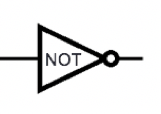
\includegraphics[height=0.5in]{../../resources/images/NOTx.png} \end{center}
\end{multicols}

%
 

{\bf Example digital circuit}: 

\begin{multicols}{2}
\begin{center}
   \includegraphics[width=1.2in]{../../resources/images/circuitEx.png} 
\end{center}
\columnbreak
Output when $x=1, y=0, z=0, w = 1$ is \underline{\phantom{$~~~0~~~$}}
Output when $x=1, y=1, z=1, w = 1$ is \underline{\phantom{$~~~0~~~$}}
Output when $x=0, y=0, z=0, w = 1$ is \underline{\phantom{$~~~0~~~$}}
\phantom{Output when $x=0, y=0, z=0, w = 0$ is \underline{\phantom{$~~~0~~~$}}}
\end{multicols}



Draw a logic circuit with inputs $x$ and $y$ whose output  is always $0$.  {\it  Can you use exactly 1 gate?}


\vspace{40pt} \newpage


{\bf Fixed-width addition}: adding one bit at time, using the usual column-by-column and carry arithmetic, and dropping the carry from the leftmost column so the result is the same width as the summands.  In many cases, this gives representation of the correct value for the sum when we interpret the summands
in fixed-width binary or in 2s complement.

For single column:
\begin{center}
\begin{tabular}{cc|cc}
\multicolumn{2}{c|}{Input}  & \multicolumn{2}{|c}{Output}  \\
$x_0$ & $y_0$ & $c_0$ & $s_0$  \\
\hline
$1$ & $1$ & \phantom{$1$} & \phantom{$0$} \\
$1$ & $0$ & \phantom{$0$} & \phantom{$1$}\\
$0$ & $1$ & \phantom{$0$} & \phantom{$1$}\\
$0$ & $0$ & \phantom{$0$} & \phantom{$0$}\\
\end{tabular}
\end{center}

\begin{center}
\includegraphics[width=1.5in]{../../resources/images/half-adder.png}
\end{center} \newpage


Draw a logic circuit that implements fixed-width 2 binary addition:
\begin{itemize}
\item Inputs  $x_0, y_0, x_1, y_1$ represent $(x_1  x_0)_{2,2}$ and $(y_1 y_0)_{2,2}$
\item Outputs  $z_0, z_1, z_2$ represent $(z_2  z_1 z_0)_{2,3} = (x_1  x_0)_{2,2} + (y_1 y_0)_{2,2}$ (may require up to width  $3$)
\end{itemize}

{\it First approach}: half-adder for each column, then combine carry from right column with sum of left column


Write expressions for the circuit output values in terms of input values:

$z_0 = \underline{\phantom{x_0 \oplus y_0\hspace{3in}}}$

$z_1 = \underline{\phantom{(x_1 \oplus y_1) \oplus c_0}\hspace{2.5in}}$ \phantom{where $c_0 = x_0 \land y_0$}

$z_2 = \underline{\phantom{(c_0 \land (x_1 \oplus y_1)) \oplus c_1}\hspace{2in}}$ \phantom{where $c_1 = x_1 \land y_1$}\\

\includegraphics[width=1.7in]{../../resources/images/width-2-adder.png}



{\it Second approach}: for middle column, first add carry from right column to $x_1$, then add result to $y_1$


Write expressions for the circuit output values in terms of input values:

$z_0 = \underline{\phantom{x_0 \oplus y_0}\hspace{3in}}$

$z_1 = \underline{ \phantom{(c_0 \oplus x_1) \oplus y_1}\hspace{2.4in}}$ \phantom{where $c_0 = x_0 \land y_0$}

$z_2 = \underline{\phantom{(c_0 \land x_1) \oplus ((c_0 \oplus x_1)\land y_1)}\hspace{1.5in}}$

\vfill

{\it Extra example} Describe how to generalize this addition circuit for larger width inputs.

 \newpage
\subsection*{Review: Week 2 Friday}
\begin{enumerate}
    \item {

\begin{enumerate}
    \item Consider the logic circuit
        \begin{center}
        \includegraphics[width=2in]{../../resources/images/review-circuit-1.png}
        \end{center}
        Calculate the value of the output of this circuit ($y_1$) for each of the following settings(s) of input values.
        \begin{enumerate}
            \item $x_1 = 1$, $x_2 = 1$
            \item $x_1 = 1$, $x_2 = 0$
            \item $x_1 = 0$, $x_2 = 1$
            \item $x_1 = 0$, $x_2 = 0$
        \end{enumerate}  \item Consider the logic circuit
        \begin{center}
        \includegraphics[width=2in]{../../resources/images/review-circuit-2.png}
        \end{center}
        For which of the following settings(s) of input values is the output
        $y_1 = 0$, $y_2 = 1$? (Select all and only those that apply.)
        \begin{enumerate}
            \item $x_1 = 0$, $x_2 = 0$, $x_3 = 0$, and $x_4 = 0$
            \item $x_1 = 1$, $x_2 = 1$, $x_3 = 1$, and $x_4 = 1$
            \item $x_1 = 1$, $x_2 = 0$, $x_3 = 0$, and $x_4 = 1$
            \item $x_1 = 0$, $x_2 = 0$, $x_3 = 1$, and $x_4 = 1$
        \end{enumerate}
      
    \end{enumerate}
     }
    \item {

Recall this circuit from class:
\begin{center}
    \includegraphics[width=1.2in]{../../resources/images/circuitEx.png} 
 \end{center}

 Which of the following is true about all possible 
 input values $x,y,z,w$? (Select all and only 
 choices that are true for all values.)
 \begin{enumerate}
    \item The output $out$ is set to $1$ exactly when $x$ is $0$,
    and it is set to $0$ otherwise.
    \item The output $out$ is set to $1$ exactly when  $(xyzw)_{2,4} < 8$,
    and it is set to $0$ otherwise.
    \item The output $out$ is set to $1$ exactly when  $(wzyx)_{2,4}$
    is an even integer,
    and it is set to $0$ otherwise.
 \end{enumerate} }
\end{enumerate}
\end{document}
